\documentclass{article}
\linespread{1.3}
\usepackage[margin=50pt]{geometry}
\usepackage{amsmath, amsthm, amssymb, amsthm, tikz, fancyhdr}
\pagestyle{fancy}
\renewcommand{\headrulewidth}{0pt}
\newcommand{\changefont}{\fontsize{15}{15}\selectfont}

\fancypagestyle{firstpageheader}
{
  \fancyhead[R]{\changefont Michael Huang \\ CFRM 415 \\ Final}
}

\begin{document}

\thispagestyle{firstpageheader}

\section*{1.}
{\Large 

We aim to find the minimium variance portfolio, as described. We form the matrix version of the Lagrangian, which is \\
$\mathcal{L} (\omega, \lambda_1, \lambda_2) = f(x) + \lambda_1 g(x) + \lambda_2 h(x)$ \\
for $g(x) = 0, h(x) = 0$. We have $f(x) = \frac{1}{2}\omega^T \Sigma \omega$, $g(x) = \omega^T 1 = 1$, and $h(x) = \omega^T \mu = \mu_p$, so we can effectively modify this equation to be \\
$\mathcal{L} (\omega, \lambda_1, \lambda_2) = \frac{1}{2}\omega^T \Sigma \omega + \lambda_1 (1 - \omega^T 1) + \lambda_2 (\mu_p - \omega^T \mu)$ \\
We take the derivatives, giving us the following: \\ \\
$\frac{\partial \mathcal{L}}{\partial \omega} = \omega^T\Sigma - \lambda_1(1) - \lambda_2(\mu) = \Sigma\omega - \lambda_11 - \lambda\mu = 0$ \\ 
$\frac{\partial \mathcal{L}}{\partial \lambda_1} = 1 - \omega^T1 = 0$ \\
$\frac{\partial \mathcal{L}}{\partial \lambda_2} = \mu_p - \omega^T\mu = 0$ \\ \\
We can use the first derivative we took to find that for $\omega^*$, we have \\
$0 = \Sigma\omega^* - \lambda_11 - \lambda_2\mu$ \\
$\lambda_11 + \lambda\mu = \Sigma\omega^*$ \\
$\Sigma^{-1}(\lambda_11 + \lambda_2\mu) = \omega^*$ \\
$\omega^* = \Sigma^{-1}(\lambda_11 + \lambda_2\mu)$ \\
exactly as we sought to show. \\ \\
To verify the values of $\lambda_1$ and $\lambda_2$, we use the latter two derivatives and substitute our solution to $\omega$: \\ \\
$1 = \omega^T1$ \\
$\mu_p = \omega^T\mu$ \\ \\
$1 = (\Sigma^{-1}(\lambda_11 + \lambda_2\mu))^T1$ \\
$\mu_p = (\Sigma^{-1}(\lambda_11 + \lambda_2\mu))^T\mu$ \\ \\
$1 = (\lambda_1\Sigma^{-1}1 + \lambda_2\Sigma^{-1}\mu)^T1$ \\
$\mu_p = (\lambda_1\Sigma^{-1}1 + \lambda_2\Sigma^{-1}\mu)^T\mu$ \\ \\
$1 = (\lambda_11^T\Sigma^{-1} + \lambda_2\mu^T\Sigma^{-1})1$ \\
$\mu_p = (\lambda_11^T\Sigma^{-1} + \lambda_2\mu^T\Sigma^{-1})\mu$ \\ \\
$1 = \lambda_11^T\Sigma^{-1}1 + \lambda_2\mu^T\Sigma^{-1}1$ \\
$\mu_p = \lambda_11^T\Sigma^{-1}\mu + \lambda_2\mu^T\Sigma^{-1}\mu$ \\ \\
$1 = \lambda_11^T\Sigma^{-1}1 + \lambda_21^T\Sigma^{-1}\mu$ \hfill By property of transpose and symmetry of $\Sigma$ \\
$\mu_p = \lambda_11^T\Sigma^{-1}\mu + \lambda_2\mu^T\Sigma^{-1}\mu$ \\ \\
We can rearrange this as a system of equations in matrix form: \\
$\begin{bmatrix}
  1 \\
  \mu_p
\end{bmatrix}
= 
\begin{bmatrix}
  A & B \\
  B & C
\end{bmatrix}
\begin{bmatrix}
  \lambda_1 \\
  \lambda_2
\end{bmatrix}$ \\ \\
We can easily verify at this point that $A = 1^T\Sigma^{-1}1, B = 1^T\Sigma^{-1}u, C = \mu^T\Sigma^{-1}\mu$ as we aimed to show. We can then solve for $\lambda_1, \lambda_2$: \\ \\
$\begin{bmatrix}
  1 \\
  \mu_p
\end{bmatrix}
= 
\begin{bmatrix}
  A & B \\
  B & C
\end{bmatrix}
\begin{bmatrix}
  \lambda_1 \\
  \lambda_2
\end{bmatrix}$ \\ \\
$\begin{bmatrix}
  1 \\
  \mu_p
\end{bmatrix}
= 
\begin{bmatrix}
  \lambda_1A +\lambda_2B \\
  \lambda_1B + \lambda_2C
\end{bmatrix}$ \\ \\
$1 = \lambda_1A + \lambda_2B$ \hfill Convert back to system of equations \\
$\mu_p = \lambda_1B + \lambda_2C$ \\ \\
$\frac{1 - \lambda_2B}{A} = \lambda_1$ \\ \\
% $\mu_p = \lambda_1B + \lambda_2C$ \\ \\
% $\frac{1 - \lambda_2B}{A} = \lambda_1$ \\
$\mu_p = \frac{1 - \lambda_2B}{A}B + \lambda_2C$ \hfill Substitute $\lambda_1$ into other equation \\
$\mu_p = \frac{B}{A} - \lambda_2\frac{B^2}{A} + \lambda_2C$ \\
$\mu_p - \frac{B}{A} =  \lambda_2 (C - \frac{B^2}{A})$ \\ 
$\frac{A\mu_p - B}{A} =  \lambda_2 (\frac{AC - B^2}{A})$ \\
$\frac{A\mu_p - B}{AC - B^2} =  \lambda_2$ \\ \\
$\frac{1 - \frac{A\mu_p - B}{AC - B^2}B}{A} =  \lambda_1$ \hfill Substitute $\lambda_2$ back into first equation \\
$\frac{\frac{AC - B^2 - AB\mu_p + B^2}{AC - B^2}}{A} =  \lambda_1$ \\
$\frac{\frac{AC - AB\mu_p}{AC - B^2}}{A} =  \lambda_1$ \\
$\frac{C - B\mu_p}{AC - B^2} =  \lambda_1$ \\
which confirms both values of $\lambda$ that we aimed to show.

\newpage
}

\section*{2.}
{\Large

\textbf{I wrote the tree calculations out in python, so as to avoid confusing myself, and rounded to account for the floating-point error}

\begin{verbatim}

import math
import numpy as np

up_p = 0.525
down_p = 1 - up_p
up = 1.152
down = 0.868
discount = math.e ** (-0.05 * 0.5)
s = 990
k = 1000

is_american = True

def main():
  price_tree = np.zeros((7, 4))
  payoff_tree = np.zeros((7, 4))

  rows, cols = price_tree.shape
  
  # initialize price
  price_tree[3][0] = s
  
  cur_ind_list = [3]
  for i in range(1, cols):
    for j in range(rows):
      if j - 1 >= 0 and price_tree[j - 1][i - 1] != 0:
        price_tree[j][i] = price_tree[j - 1][i - 1] * down
      if j + 1 <= rows - 1 and price_tree[j + 1][i - 1] != 0:
        price_tree[j][i] = price_tree[j + 1][i - 1] * up

  # initialize payoffs after pricing
  for i in np.arange(6, -1, -1):
    if price_tree[i][3] == 0:
      continue

    if price_tree[i][3] < k:
      payoff_tree[i][3] = k - price_tree[i][3]
    else:
      payoff_tree[i][3] = 0

  # start traversing backwards and replace accordingly
  for i in np.arange(cols - 2, -1, -1):
    for j in range(1, rows - 1):
      if price_tree[j + 1][i + 1] != 0 and price_tree[j - 1][i + 1] != 0:
        up_factor = payoff_tree[j - 1][i + 1] * up_p
        down_factor = payoff_tree[j + 1][i + 1] * down_p
        payoff_tree[j][i] = discount * (up_factor + down_factor)
      
      if is_american:
        # replace as necessary in american case
        exercise = k - price_tree[j][i]
        if price_tree[j][i] != 0 and payoff_tree[j][i] < exercise:
          print("crossed out " + str(payoff_tree[j][i]) + " for " + str(exercise))
          payoff_tree[j][i] = exercise

  # formula: discount * ((u_p * up_val) + (d_p * down_val))

  print("price_tree")
  print(price_tree)
  print("payoff_tree")
  print(payoff_tree)
  

if __name__ == "__main__":
  main()

\end{verbatim}

\newpage

\subsection*{(a)}

$S_0 = 990, r = 0.05, q = 0.02, K = 1000, \sigma = 0.20, \delta t = 0.5$, since 18 months is 1.5 years, and $1.5 / 3 = 0.5$. Note that we use $K$ rather than $X$ as the strike price here. \\
We have that \\
$u = e^{\sigma\sqrt{\delta t}} = e^{0.2 \cdot \sqrt{0.5}} = \sim 1.152$ \\
$d = \frac{1}{u} = e^{-\sigma\sqrt{\delta t}} = e^{-0.2 \cdot \sqrt{0.5}} = \sim 0.868$ \\
$p = \frac{R - d}{u - d} = \frac{e^{(0.05 - 0.02) \cdot 0.5} - e^{-0.2 \cdot \sqrt{0.5}}}{e^{0.2 \cdot \sqrt{0.5}} - e^{-0.2 \cdot \sqrt{0.5}}} = \frac{1}{2} + \frac{1}{2}(\frac{0.05 - 0.02 - \frac{1}{2}0.20^2}{0.20}) = 0.525$ \\ \\
As we can see in the diagram, the final value is \framebox[1.1\width]{$\mathbf{\sim \$ 85.46932493}$}

\begin{figure}[h]
  \centering
  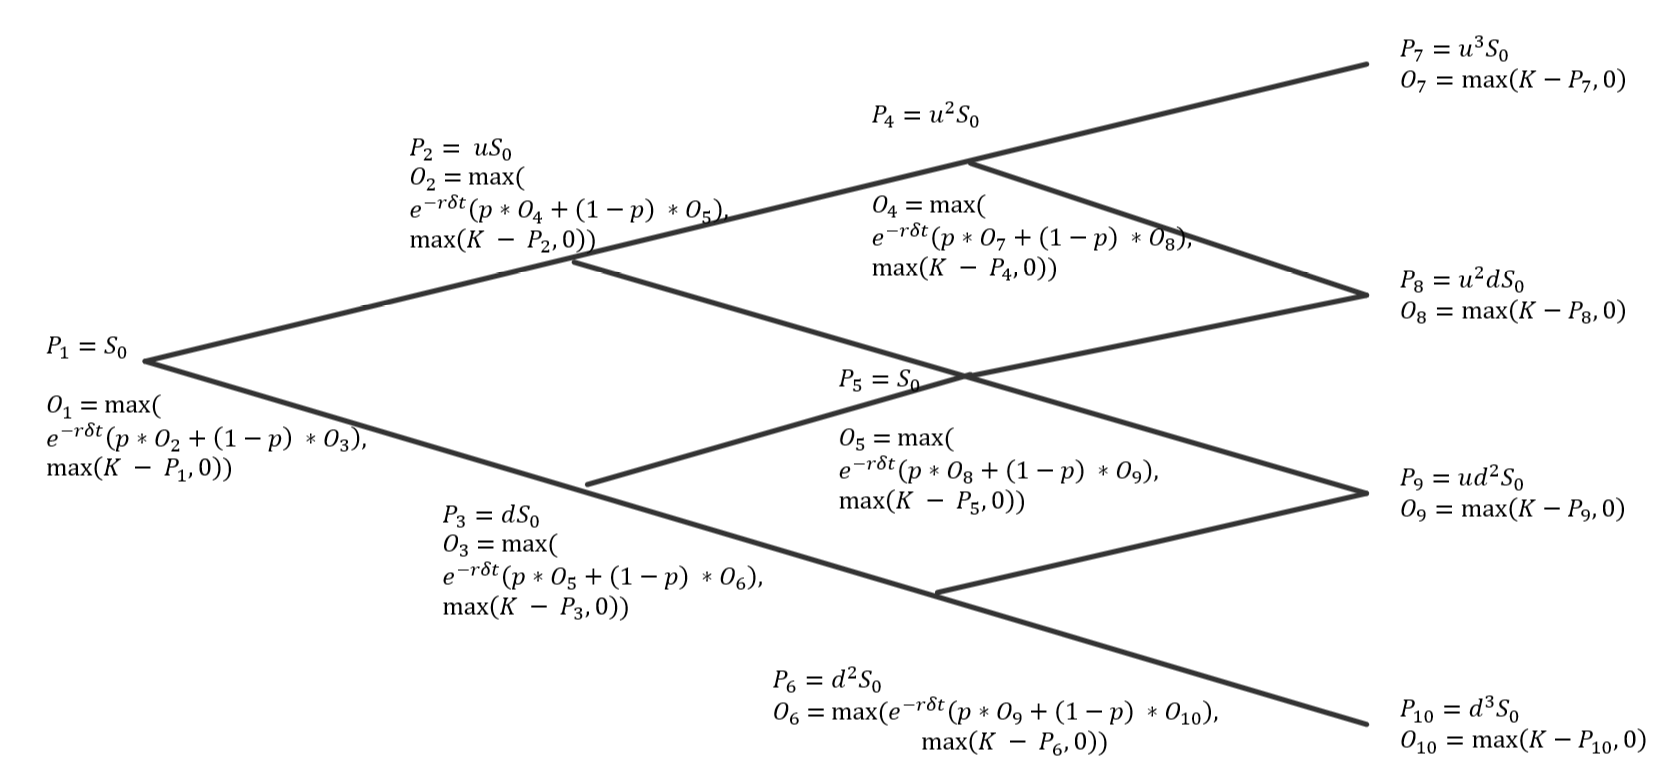
\includegraphics[width=120mm]{./2a_tree.png}
\end{figure}

All calculations were then automated in python. Note that we use $K$ rather than $X$ as the strike price here, and $P$ as the stock price and $O$ as the option value.

\begin{figure}[h]
  \centering
  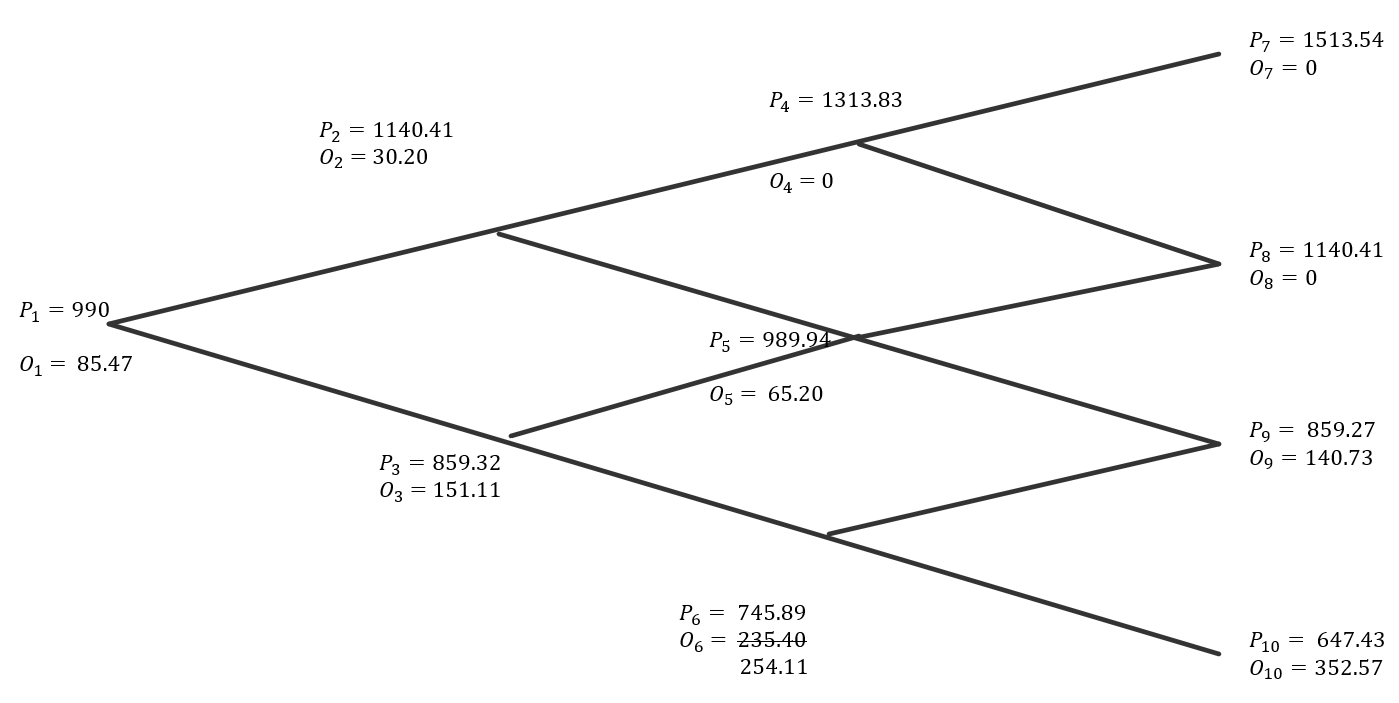
\includegraphics[width=120mm]{./2a_finaltree.png}
\end{figure}

\newpage

\subsection*{(b)}

As we compare, we can see that the starting node's value differs by $\sim 85.46932493 - \sim 81.452947 = $ \framebox[1.1\width]{$\mathbf{\sim \$ 4.01637793}$}

\begin{figure}[h]
  \centering
  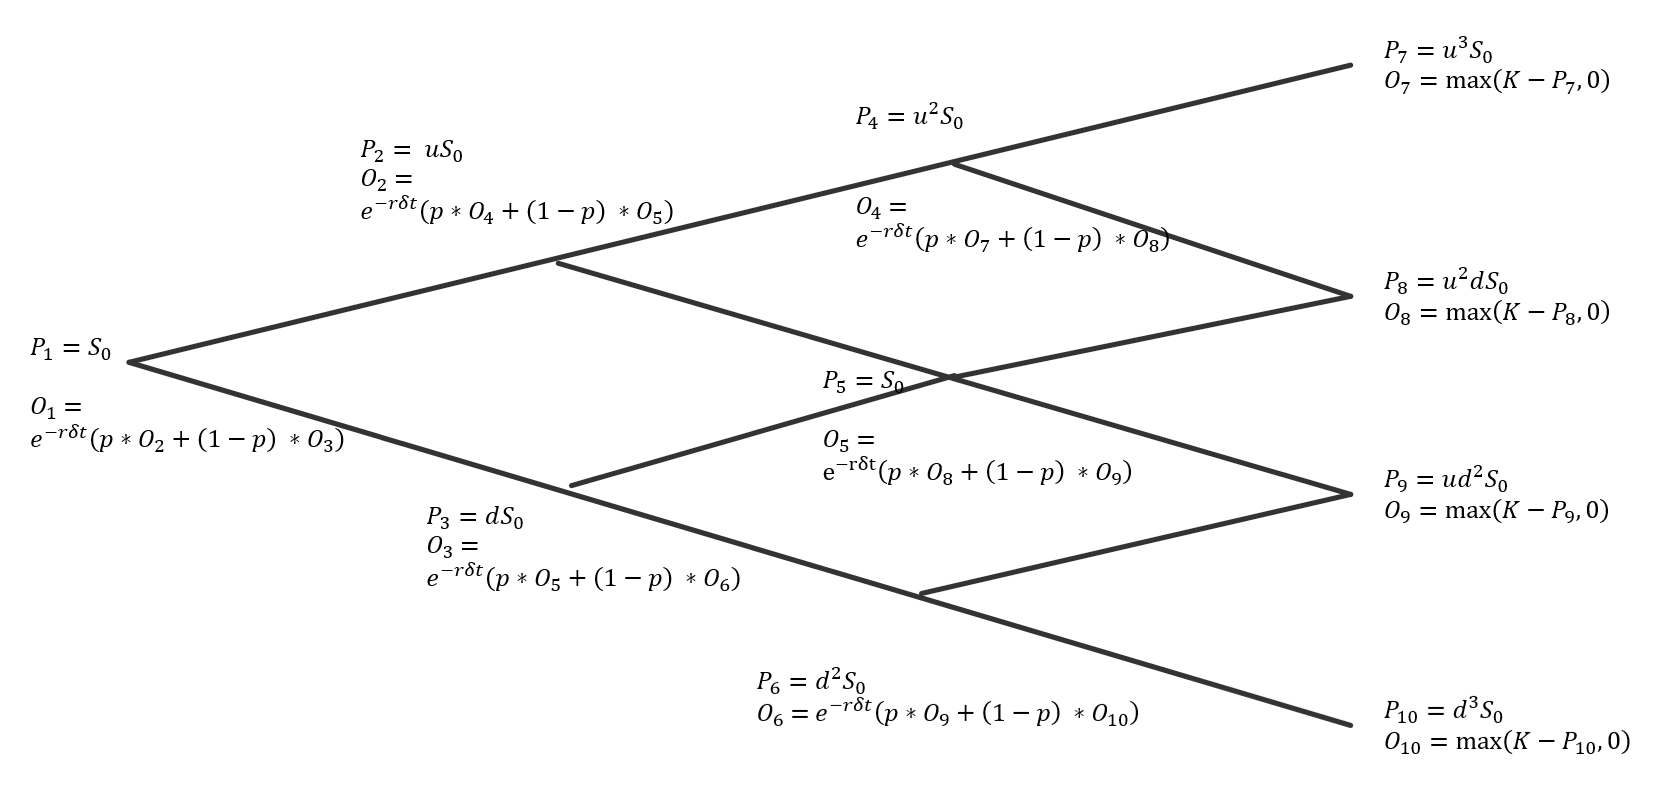
\includegraphics[width=120mm]{./2b_tree.png}
\end{figure}

All calculations were then automated in python. Note that we use $K$ rather than $X$ as the strike price here, and $P$ as the stock price and $O$ as the option value.

\begin{figure}[h]
  \centering
  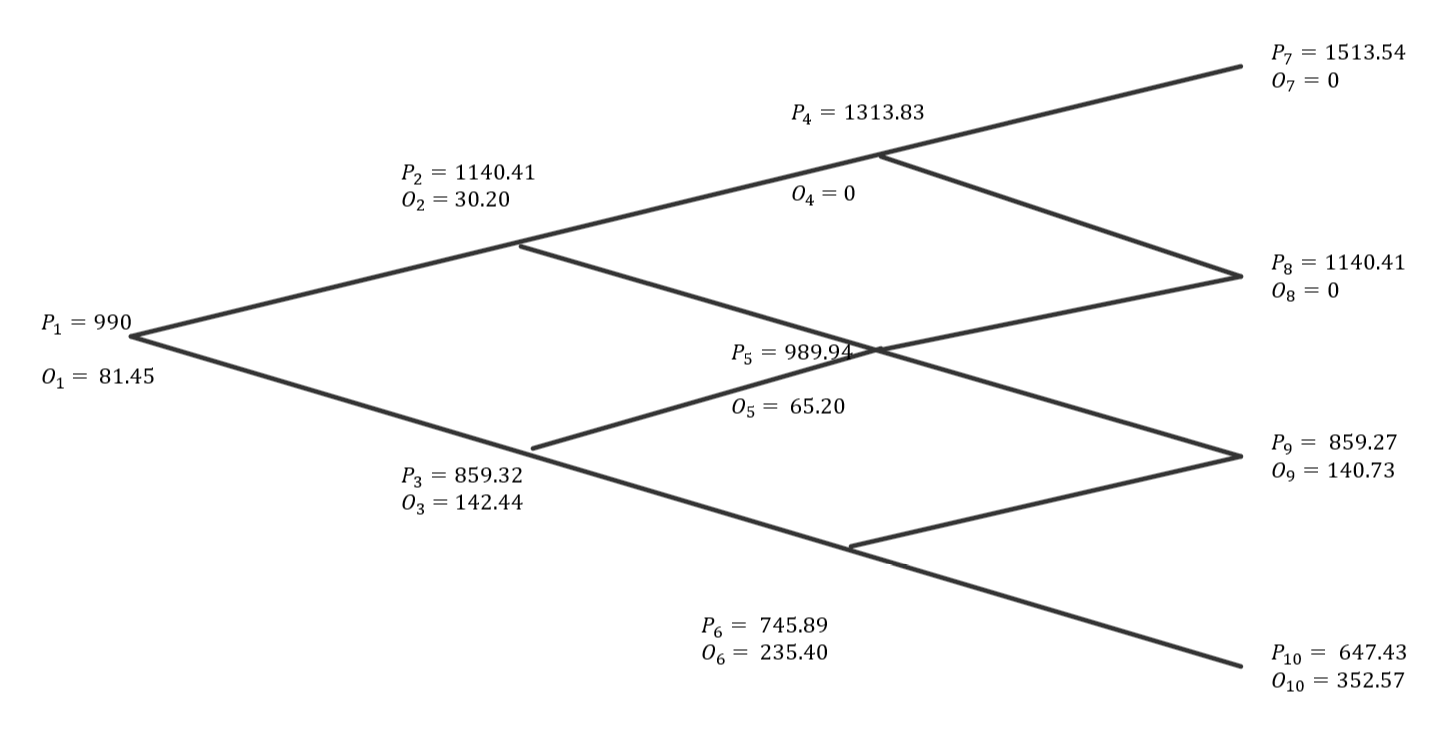
\includegraphics[width=120mm]{./2b_finaltree.png}
\end{figure}

\subsection*{(c)}

% Suppose we chop the same time to expiration up into much smaller time steps for this binomial lattice, and we find the price for 149 time steps to 84, 150 time steps to be 85, and 151 time steps to be 86. What should we take as the option premium in this case? \\ \\

% We know that for a put, the option premium = $(X - S)^+ + \text{time value}$. We note that we are deep ITM, so we can say that $P^{AM} = X - S$ since we have time value of $0$, so all that is left is $X - S = 1000 - 990 = $ \framebox[1.1\width]{$\mathbf{\$ 10}$}. 

In class, we noted that at about 150 steps, we have an answer that is close enough for commercial purposes, and is a good average in between the given options. Therefore, \framebox[1.1\width]{$\mathbf{85}$} is likely a good option premium to take.

\newpage
}

\section*{3.}
{\Large 

\subsection*{(a)}

We calculate the count-adjusted year fraction to be $0.063889$. \\
$S = 3200, X = 3150, T-t = 0.063889, r = 0.01, \sigma = 0.30$ \\ \\
$C(S, T) = SN(d_1) - Xe^{-r(T-t)}N(d_2)$ \\
$d_1 = \frac{log(\frac{S}{X}) + (r+\frac{1}{2}\sigma^2)(T-t)}{\sigma\sqrt{T-t}}$ \\
$d_2 = d_1 - \sigma\sqrt{T-t}$ \\ \\
We use python to perform the raw calculations yet again:
\begin{verbatim}
import math
import numpy as np
from scipy.stats import norm

S = 3200
X = 3150
time = 0.063889
r = 0.01
sigma = 0.30

d_1 = (math.log(S / X) + ((r + 0.5 * (sigma ** 2)) * (time))) / 
(sigma * np.sqrt(time))
d_2 = d_1 - (sigma * np.sqrt(time))

call = (S * norm.cdf(d_1)) 
- (X * (math.e ** (-r * time)) * norm.cdf(d_2))

print("call")
print(call)
\end{verbatim}
\framebox[1.1\width]{$\mathbf{124.23224257130119}$}

\subsection*{(b)}

Via put-call parity with no dividend, we know that it is never optimal to exercise an American call option, i.e. it is best to close the position rather than exercise, which means that we can say that it has the same price as the European call option, that is, \framebox[1.1\width]{$\mathbf{124.23224257130119}$}

\subsection*{(c)}

We keep the same $d_1$ and $d_2$, and know that the formula for put is $P(S, t) = Xe^{-r(T - t)}N(-d_2) - SN(-d_1)$ \\
We turn to python to perform the raw calculations yet again:
\begin{verbatim}
import math
import numpy as np
from scipy.stats import norm

S = 3200
X = 3150
time = 0.063889
r = 0.01
sigma = 0.30

d_1 = (math.log(S / X) + ((r + 0.5 * (sigma ** 2)) * (time))) / 
(sigma * np.sqrt(time))
d_2 = d_1 - (sigma * np.sqrt(time))

put = (X * (math.e ** (-r * time)) * norm.cdf(-d_2)) 
- (S * norm.cdf(-d_1))

print("put")
print(put)
\end{verbatim}
\framebox[1.1\width]{$\mathbf{72.22038181859284}$}
\newpage
}

\section*{4.}
{\Large 

\subsection*{(a)}
We know that with $t_0 = 0$, $P(t, T) = P(0, T) / P(0, t)$, or that \\
$P(0, T) = P(t, T) \cdot P(0, t)$: \\ \\
$P(T_0, T_2) = P(T_1, T_2) \cdot P(T_0, T_1) = 0.940 \cdot 0.950 = $ \framebox[1.1\width]{$\mathbf{0.893}$} \\ 
$P (T_0, T_3) = P(T_2, T_3) \cdot P(T_0, T_2) = 0.932 \cdot 0.893 = $ \framebox[1.1\width]{$\mathbf{0.832276}$} \\
$P(T_0, T_4) = P(T_3, T_4) \cdot P(T_0, T_3) = 0.925 \cdot 0.832276 = $ \framebox[1.1\width]{$\mathbf{0.7698553}$} \\
$P(T_0, T_5) = P(T_4, T_5) \cdot P(T_0, T_4) = 0.919 \cdot 0.7698553 = $ \framebox[1.1\width]{$\mathbf{0.7074970207}$} \\
$P(T_0, T_6) = P(T_5, T_6) \cdot P(T_0, T_5) = 0.913 \cdot 0.7074970207 =  $ \framebox[1.1\width]{$\mathbf{0.64594477989}$}

\subsection*{(b)}

Since each discount rate is annual, we know that the year-count difference between any two adjacent $T_i$ is 1, and adapt this accordingly between $T_0$ and $T_i$: \\ $R(t, T) := -ln(P(t, T)) / \tau(t, T)$ \\ \\
$R(T_0, T_1) = -ln(P(T_0, T_1)) / \tau(T_0, T_1) = -ln(0.950) / 1 = $ \framebox[1.1\width]{$\mathbf{0.05129329438}$} \\
$R(T_0, T_2) = -ln(P(T_0, T_2)) / \tau(T_0, T_2) = -ln(0.893) / 2 = $ \framebox[1.1\width]{$\mathbf{0.05658434905}$} \\
$R(T_0, T_3) = -ln(P(T_0, T_3)) / \tau(T_0, T_3) = -ln(0.832276) / 3 = $ \framebox[1.1\width]{$\mathbf{0.06119705413}$} \\
$R(T_0, T_4) = -ln(P(T_0, T_4)) / \tau(T_0, T_4) = -ln(0.7698553) / 4 = $ \framebox[1.1\width]{$\mathbf{0.06538817596}$} \\
$R(T_0, T_5) = -ln(P(T_0, T_5)) / \tau(T_0, T_5) = -ln(0.7074970207) / 5 = $ \framebox[1.1\width]{$\mathbf{0.06920437209}$} \\
$R(T_0, T_6) = -ln(P(T_0, T_6)) / \tau(T_0, T_6) = -ln(0.64594477989) / 6 = $ \framebox[1.1\width]{$\mathbf{0.07284020981}$} \\


}

\end{document}